
\section{Experiments}
\label{sec:experiments}

In this section, we present three sets of experiments on the NCAA basketball
dataset: 1. event classification, 2. event detection and 3. evaluation of
attention

\eat{
. Note that previous attention models have typically shown selected
qualitative results to visualize attention in their settings. However, few
attempts have been made to quantitatively evaluate attention. A key
contribution of our paper is to provide both a qualitative and a quantitative
analyis of the attention scores.
}

\subsection{Implementation details}

 We used a hidden state dimension of $256$ for all the LSTM and
BLSTM RNNs, an embedding layer with ReLU non-linearity and $256$ dimension for
embedding the player features and frame features before feeding to the RNNs.
We used $32 \times 32$ bins with spatial pyramid pooling for the player appearance
feature.
All the event videos clips were four seconds long and subsampled to 6fps.  The
$\tau$ value was set to $0.25$ for the attention softmax weighting. We used a
batch size of $128$, learning rate of $0.005$ which was reduced by a factor of
$0.1$ every $10000$ iterations with RMSProp\cite{RMSProp}. The models were trained on
a cluster of $20$ GPUs for $100k$ iterations over one day.
The hyperparameters were chosen by cross-validating on the
validation set.

\subsection{Event classification}

In this section, we compare the ability of methods to perform 11-way classification of isolated video clips.
In this setting, we do not use any
additional negatives from other parts of the basketball videos.
We compare our results
against different control settings and baseline models as explained
below:


\begin{table*}[t!]
\begin{center}
\small
 \begin{tabular}{|l|c|c|c|c|c|c|c|c|c|}
  \hline
Event & IDT\cite{Wang_CVPR11} & IDT\cite{Wang_CVPR11} player & C3D \cite{Tran_arxiv14} & LRCN \cite{Donahue_arxiv14} & MIL\cite{} & Only player & Avg. player & Our no track & Our with track \\ \hline \hline

3-point succ.    & 0.501 & 0.481 & 0.282 & 0.462 &  & 0.469 & 0.545 & 0.583 & 0.600 \\
3-point fail.    & 0.370 &  0.428& 0.117 & 0.564 &  & 0.614 & 0.702 & 0.668 & 0.738 \\
fr-throw succ. & 0.365 &  0.623& 0.319 & 0.876 &  & 0.885 & 0.809 & 0.892 & 0.882 \\
fr-throw fail. & 0.778 &  0.703& 0.642 & 0.584 &  & 0.700 & 0.641 & 0.671 & 0.516 \\
layup succ.      & 0.278 & 0.311 & 0.185 & 0.463 &  & 0.416 & 0.472 & 0.489 & 0.500 \\
layup fail.      & 0.283 &0.300  & 0.195 & 0.386 &  & 0.305 & 0.388 & 0.426 & 0.445 \\
2-point succ.    & 0.303 &  0.285 & 0.254 & 0.257 &  & 0.228 & 0.255 & 0.281 & 0.341 \\
2-point fail.    & 0.136 &  0.233 & 0.078 & 0.378 &  & 0.391 & 0.473 & 0.442 & 0.471 \\
sl. dunk succ.  & 0.004 &  0.171 & 0.004 & 0.285 &  & 0.107 & 0.186 & 0.210 & 0.291 \\
sl. dunk fail.  & 0.197 &  0.010& 0.047 & 0.027 &  & 0.006 & 0.010 & 0.006 & 0.004 \\
steal            & 0.555 &  0.473& 0.303 & 0.876 &  & 0.854 & 0.894 & 0.886 & 0.893 \\ \hline \hline
Mean             & 0.343 &  0.365 & 0.221 & 0.469 &  & 0.452 & 0.489 & 0.505 & 0.516 \\ \hline
  \end{tabular}
\end{center}
  \caption{Mean average precision for event {\em classification} given
    isolated clips.}
  \label{tab:event_class}
  \label{tab:class_res}
\end{table*}

\begin{itemize}
  \item \emph{IDT\cite{Wang_CVPR11}} We use the publicly available implementation of dense trajectories with
  Fisher encoding.
  
  \item \emph{IDT\cite{Wang_CVPR11} player} We use IDT along with averaged features extracted from the player
  bounding boxes.

  \item \emph{C3D \cite{Tran_arxiv14}} We use the publicly available pre-trained model for feature extraction
  with a SVM classifier.

  \item \emph{LRCN \cite{Donahue_arxiv14}} This is a baseline model where we use a simple BLSTM on frame-level features similar
  to LRCN. The only difference is the use of BLSTM in place of LSTM. We found this to improve
  performance.

  \item \emph{MIL \cite{}} Since each frame can be seen as a bag of player features, we used the
  classical MIL model. 

  \item \emph{Only player} We only use player features without frame-level
  features.
 
  \item \emph{Avg. player} We combine the player features by simple averaging, without
using  attention.

  \item \emph{Attn. no track} Our attention model without tracks.

  \item \emph{Attn. with track} Our attention model with tracking.
\end{itemize}

The mean average precision (mAP)
are shown in Tab.~\ref{tab:class_res}. We see that ...


\subsection{Event detection}

In this section, we evaluate the ability of methods to temporally localize events in untrimmed videos.
We use a sliding window approach, where we slide a $4$ second window
through all the basketball videos and try to classify the window into a negative
class or one of the 11 event classes. We use a stride length of $2$ seconds.
We treat all windows which do not overalp more than $1$ sec with any of the $11$ annotated
events as negatives. We use the same setting for training, test and validation.
This leads to $90200$ negative examples across all the videos.
 We compare with the same baselines as before.

\begin{table*}[ht!]
\begin{center}
\small
 \begin{tabular}{|l|c|c|c|c|c|c|c|c|c|}
  \hline
Event & IDT\cite{Wang_CVPR11} & IDT player\cite{Wang_CVPR11} & C3D \cite{Tran_arxiv14} & LRCN \cite{Donahue_arxiv14} & MIL\cite{} & Only player & Avg. player & Our no track & Our with track \\ \hline \hline
3-point succ.  &  &  &  & 0.505 &  & 0.526 & 0.521 & 0.556 & 0.600 \\
3-point fail.  &  &  &  & 0.230 &  & 0.251 & 0.268 & 0.263 & 0.239 \\
fr-throw succ. &  &  &  & 0.122 &  & 0.059 & 0.009 & 0.005 & 0.045 \\
fr-throw fail. &  &  &  & 0.741 &  & 0.777 & 0.811 & 0.788 & 0.810 \\
layup succ.    &  &  &  & 0.434 &  & 0.470 & 0.444 & 0.468 & 0.405 \\
layup fail.    &  &  &  & 0.187 &  & 0.142 & 0.139 & 0.208 & 0.208 \\
2-point succ.  &  &  &  & 0.492 &  & 0.402 & 0.489 & 0.494 & 0.512 \\
2-point fail.  &  &  &  & 0.544 &  & 0.578 & 0.684 & 0.619 & 0.674 \\
sl. dunk succ. &  &  &  & 0.352 &  & 0.371 & 0.417 & 0.366 & 0.400 \\
sl. dunk fail. &  &  &  & 0.428 &  & 0.566 & 0.457 & 0.576 & 0.555 \\
steal          &  &  &  & 0.359 &  & 0.348 & 0.313 & 0.340 & 0.339 \\ \hline \hline
Mean             &  &  &  & 0.400 &  & 0.408 & 0.414 & 0.426 & 0.435 \\ \hline
  \end{tabular}
\end{center}
  \caption{Mean average precision for event {\em detection} given
    untrimmed videos.}
  \label{tab:detection_res}
\end{table*}

 The detection results
are presented in Tab.~\ref{tab:detection_res}.
We see that  ...


\subsection{Analyzing attention}

We have seen above that attention can improve the performance of the model at tasks such as classification and detection.
In this section, we evaluate how accurate the attention models are at
identifying the key players. (Note that the models were never
explicitly trained to identify key players).

\eat{
While attention to specific players improves event detection,
the attention scores themselves carry valuable information.
We observed that the attention scores represented a 
consistent meaning across multiple videos in our dataset.
More concretely, our model often ``attends" to the person shooting the
ball at the begining of an event. We can see several visual examples
in Fig.~\ref{fig:visual_attention}, where the person shooting
the ball is highlighted by attention.}


% -------- Heat Map for youtube videos
\begin{figure*}[t!]
\begin{center}
   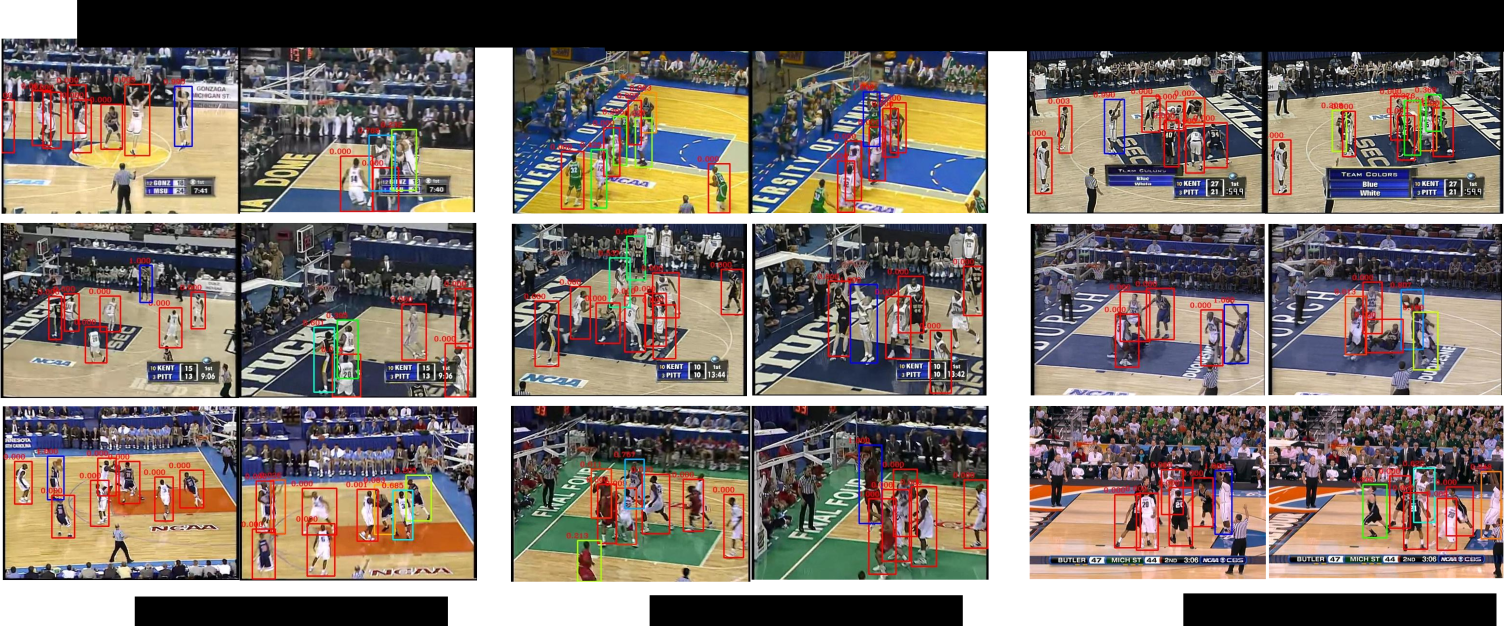
\includegraphics[width=1.0\linewidth]{images/visual_examples.pdf}
\end{center}
   \caption{Visualization of our attention scores at the begining and ending of different events.
Each row of the event corresponds to a different video. It is interesting to note that the model
attends to the shooter when the player makes a shot and to other people under the basket after
the shot is completed.}
\label{fig:visual_attention}
\end{figure*}
% ---------------------------------------------------------------------------------

To evaluate this, 
we collected AMT annotations on $850$ video clips in the test
set, where the annotators were asked to mark the position of the ball
on the frame where the shooter attempts a shot.
This provided us the location of the player shooting the ball.
We used these annotations to evaluate if our ``attention" scores
were capable of classifying the ``shooter" correctly in these frames.

\begin{table}[ht!]
\begin{center}
\small
 \begin{tabular}{|l|c|c|c|}
  \hline
Event            & Chance & Attn. no track & Attn. with track \\ \hline \hline
3-point succ.    & 0.519 & 0.333 & \\ 
3-point fail.    & 0.545 & 0.334 & \\ 
free-throw succ. & 0.772 & 0.376 & \\ 
free-throw fail. & 0.685 & 0.346 & \\  
layup succ.      & 0.627 & 0.386 & \\ 
layup fail.      & 0.605 & 0.382 & \\ 
2-point succ.    & 0.554 & 0.355 & \\ 
2-point fail.    & 0.542 & 0.346 & \\ 
slam dunk succ.  & 0.686 & 0.413 & \\ 
slam dunk fail.  & 0.645 & 0.499 & \\ \hline \hline  
Mean             & 0.377 & 0.618 & \\ \hline
  \end{tabular}
\end{center}
  \caption{Mean average precision for attention evaluation.}
  \label{tab:attention_res}
\end{table}

The mean AP for this ``shooter"  classifcation is listed
in Tab.~\ref{tab:attention_res}.
The results show that the track-free model is quite consistent in picking
the shooter for several classes like ``free-throw succ./fail",
``layup succ./fail." and ``slam dunk succ.". This is a very
promising result which shows that attention on player detections
alone is capable of localizing the player making the shot. This could be
a useful cue for providing more detailed event descriptions
including the identity and position of the shooter as well.

Another interesting observation
%from Tab.~\ref{tab:attention_res}
is that the
attention scores for the tracking based model are less selective in focusing on
the shooter.  We observed that the tracking model is often reluctant to switch
attention between frames and tends to focus on a single player throughout the
event. This biases the model towards players who are present throughout the
event. For instance, in free-throws Fig.~\ref{fig:track_spec_att} we see that
the model always attends to the defender at a specific position, who is visible
throughout the entire event unlike the shooter.

Since the identity of an event often depends on the position of the
shooter with respect to the court, we decided to evaluate the
normalized locations of the attended players.
Specifically, we annotated 5 points on the courts and
aligned all the attended boxes for an event to one cannonical image. 
Fig.~\ref{fig:att_heatmap} shows a heatmap  showing the spatial distributions
of the attended players with respect to the court. It is interesting to note that
our model consistenly focuses under the basket for a layup, at the free-throw
line for free-throws and outside the 3-point ring for 3-pointers.

\eat{
Since basketball shots are often classified based on the position of the
shooter with respect to the court, we analyze this in
Fig.~\ref{fig:att_heatmap}.  We annotated specific points on the courts and
aligned all the attended boxes for an event to one cannonical image. We have
plotted the resulting heatmap showing the distribution in position of the
attended player with respect to the court. It is interesting to note that
our model consistenly focuses under the basket for a layup, at the free-throw
line for free-throws and outside the 3-point ring for 3-pointers.
}


% -------- Heat Map for youtube videos
\begin{figure*}[t!]
\begin{center}
  \includegraphics[width=7 in]{images/attention_heatmap_full.pdf}
\end{center}
   \caption{We show the distribution of the attention over the basketball court
     for different events. We used an affine transform to transform the
     attended player's position to a cannonical frame for visualization.
     Interestingly, the attended court positions are the typical spots from
     which a player would make a shot for the corresponding event.
     \KEVIN{Also add basketball positions.}
   }
\label{fig:att_heatmap}
\end{figure*}
% ---------------------------------------------------------------------------------


